\section{Suporte à Anotação Semântica}\label{4-grasews-suporte-anotacao}

Grasews provê recursos para que o usuário seja capaz de anotar semanticamente uma especificação WSDL. Por meio de menus de contexto, o usuário é capaz de criar anotações utilizando tanto o atributo \textit{Model Reference} quanto os atributos \textit{Lifting Schema Mapping} e \textit{Lowering Schema Mapping}, do padrão SAWSDL.

A \figurename~\ref{fig:grasews} ilustra a interface gráfica de Grasews, contendo os três principais componentes visuais de Grasews. Ao centro, encontra-se o painel de visualização tanto do grafo quanto do código WSDL/XML, apresentado na seção \ref{4-grasews-grafo}. À esquerda, encontra-se o painel de visualização de elementos de uma especificação WSDL no formato de menu de árvore (\textit{tree-view}), apresentado na seção \ref{4-menu-wsdl}. Por fim, à direita, encontra-se o painel de visualização de classes de uma ontologia OWL também no formato de menu de árvore (\textit{tree-view}), apresentado na seção \ref{4-menu-owl}.

\subsection{Grafo com Suporte à Anotação Semântica}\label{4-grasews-grafo}

O principal componente visual de Grasews é o grafo. Grasews utiliza a notação visual proposta no Capítulo \ref{3-notacao-visual-para-sawsdl} para representar hierarquicamente elementos de uma especificação WSDL e classes de uma ontologia OWL, possibilitando que um usuário crie anotações semânticas segundo a abordagem SAWSDL. Para os elementos WSDL/XSD passíveis de serem anotados com \textit{Model Reference}, Grasews disponibiliza um menu de contexto para adicionar e remover um URI de \textit{Model Reference}. Para os elementos passíveis de serem anotados tanto com \textit{Model Reference} quanto com \textit{Lifting Schema Mapping} e \textit{Lowering Schema Mapping}, Grasews estende o menu de contexto anterior com opções adicionais para permitir todos os tipos de anotações. A \figurename~\ref{fig:grasews-grafo-tipo-complexo-contexto} ilustra o menu de contexto disponível para um tipo complexo XSD \texttt{GetAllBooks} (parcialmente visível atrás do menu de contexto).

A \figurename~\ref{fig:grasews-grafo-model-reference} apresenta parte do grafo de uma especificação WSDL anotada com \textit{Model Reference}. Observa-se que a interface \texttt{MyWebSerice} está anotada com \textit{Model Reference} utilizando a classe OWL \texttt{ExpressionContent}, esta pertencente à ontologia \texttt{books}. Adicionalmente, a operação \texttt{MyMethodB} está anotada com \textit{Model Reference} utilizando a classe OWL \texttt{Article}, da mesma ontologia. Grasews constrói automaticamente a estrutura hierárquica entre as duas classes OWL em uso por anotações semânticas. Com isso, as classes OWL intermediárias \texttt{LinguisticExpression} e \texttt{Text} são automaticamente dispostas no grafo entre as duas classes OWL \texttt{ExpressionContent} e \texttt{Article}.

\begin{landscape}
    \begin{figure}[h]
        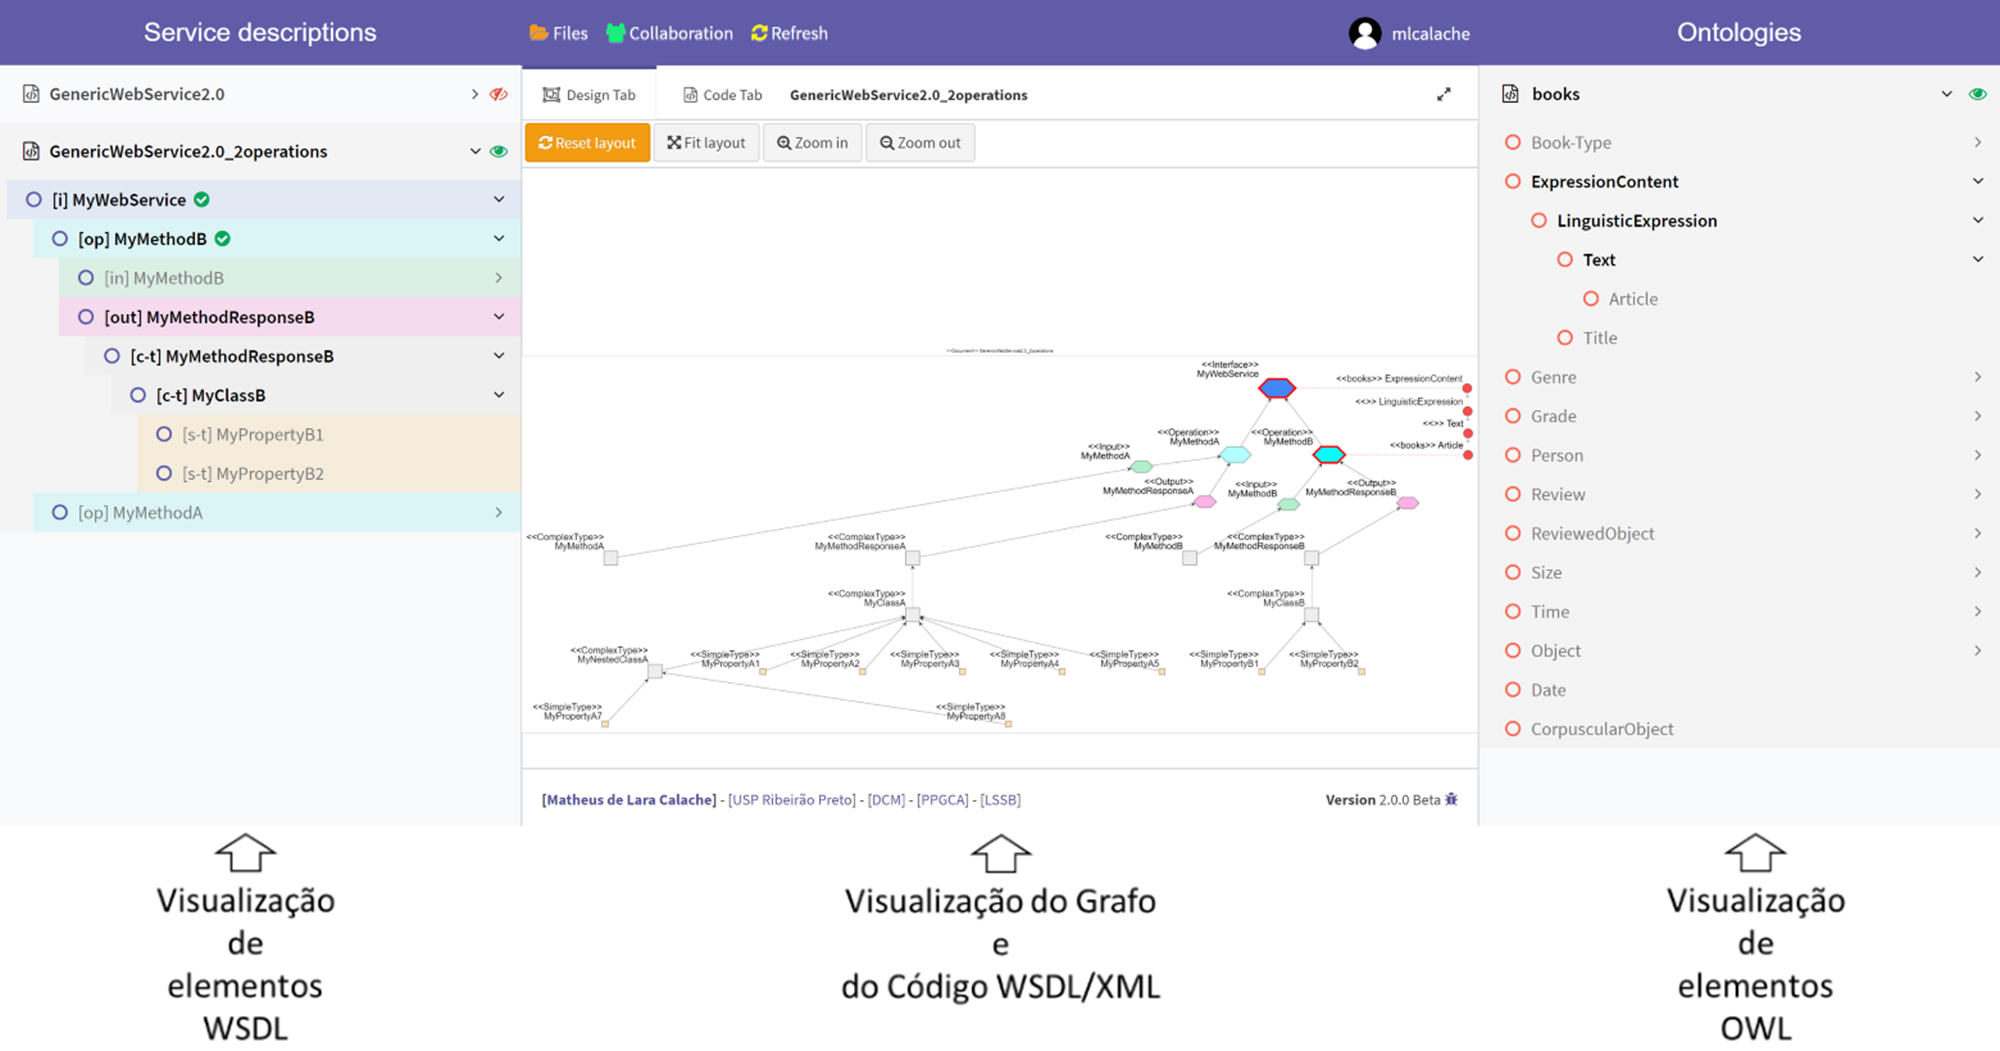
\includegraphics[scale=0.45]{4-grasews/imagens/grasews.png}
        \centering
        \caption[Interface gráfica de Grasews]{\textbf{Interface gráfica de Grasews.}}
        \label{fig:grasews}
    \end{figure}
\end{landscape}

Adicionalmente, Grasews provê um painel para visualizar o código XML de uma especificação WSDL. A \figurename~\ref{fig:grasews-painel-codigo} ilustra o painel de visualização do código WSDL/XML. O painel é automaticamente atualizado conforme o trabalho (anotações semânticas) é realizado. Com isso, caso o usuário tenha conhecimento técnico no código XML de uma especificação WSDL, este usuário pode verificar o painel de código a fim de validar as anotações semânticas criadas com o auxílio das notações visuais de Grasews. Entretanto, o painel de visualização de código não é editável.

\begin{figure}[h]
    %\resizebox{\textwidth}{!}{
        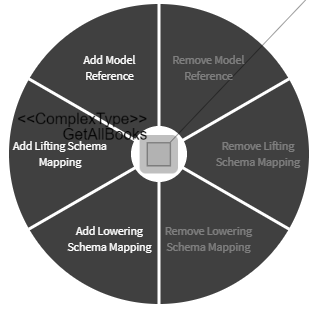
\includegraphics[scale=0.8]{4-grasews/imagens/grasews-grafo-tipo-complexo-contexto.png}
    %}
    \centering
    \caption[Menu de contexto para anotação semântica por meio do grafo de Grasews]{\textbf{Menu de contexto para anotação semântica por meio de grafo do Grasews.}}
    \label{fig:grasews-grafo-tipo-complexo-contexto}
\end{figure}

\begin{figure}[h]
    \resizebox{\textwidth}{!}{
        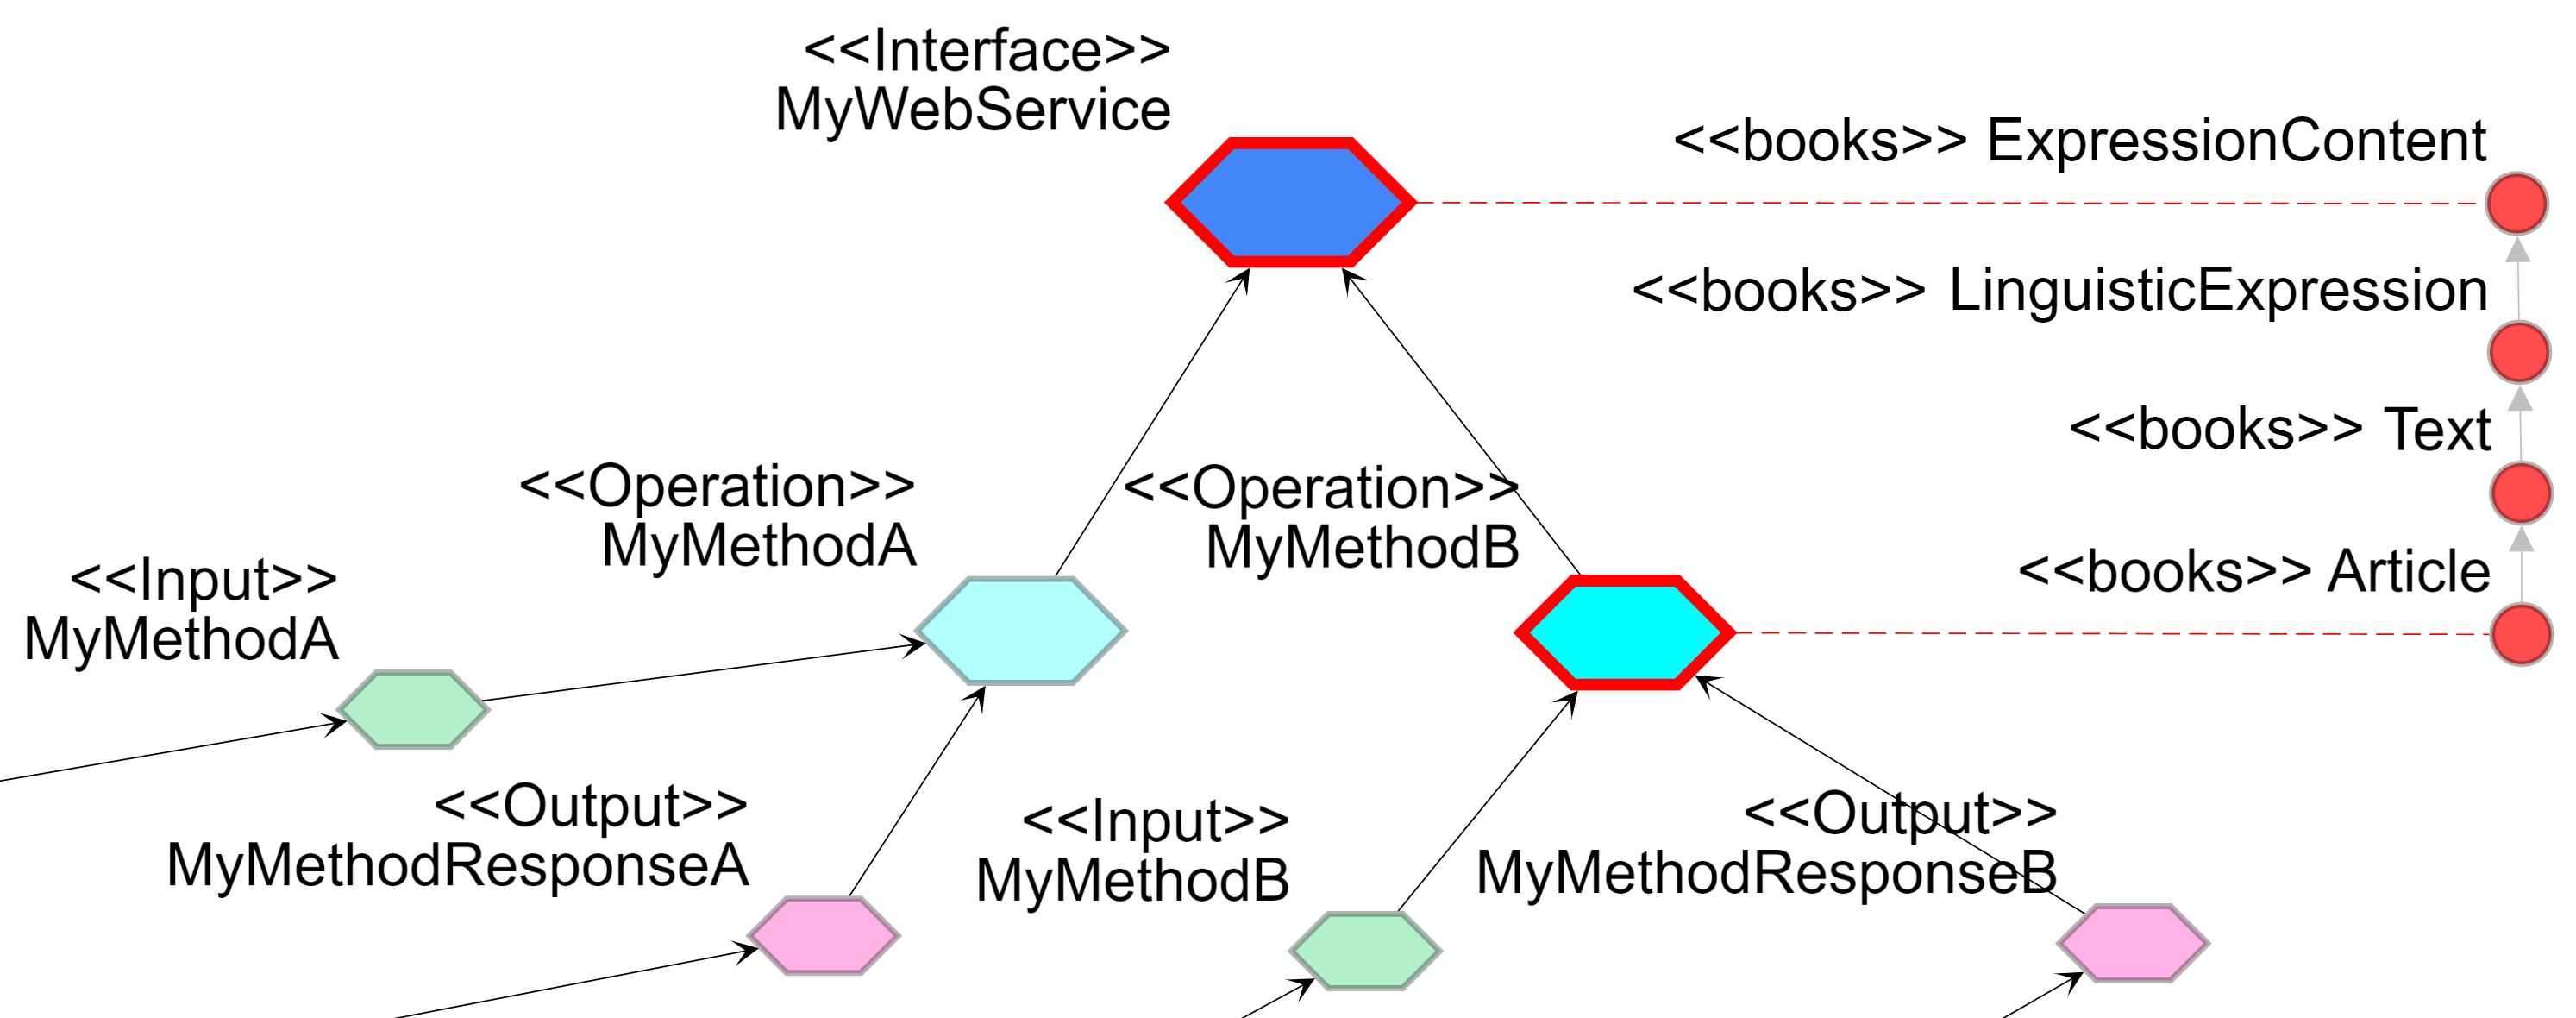
\includegraphics[scale=0.8]{4-grasews/imagens/grasews-grafo-model-reference.png}
    }
    \centering
    \caption[Elementos do grafo de Grasews anotados com \textit{Model Reference}]{\textbf{Elementos do grafo de Grasews anotados com \textit{Model Reference}.}}
    \label{fig:grasews-grafo-model-reference}
\end{figure}

\begin{figure}[h]
    \resizebox{\textwidth}{!}{
        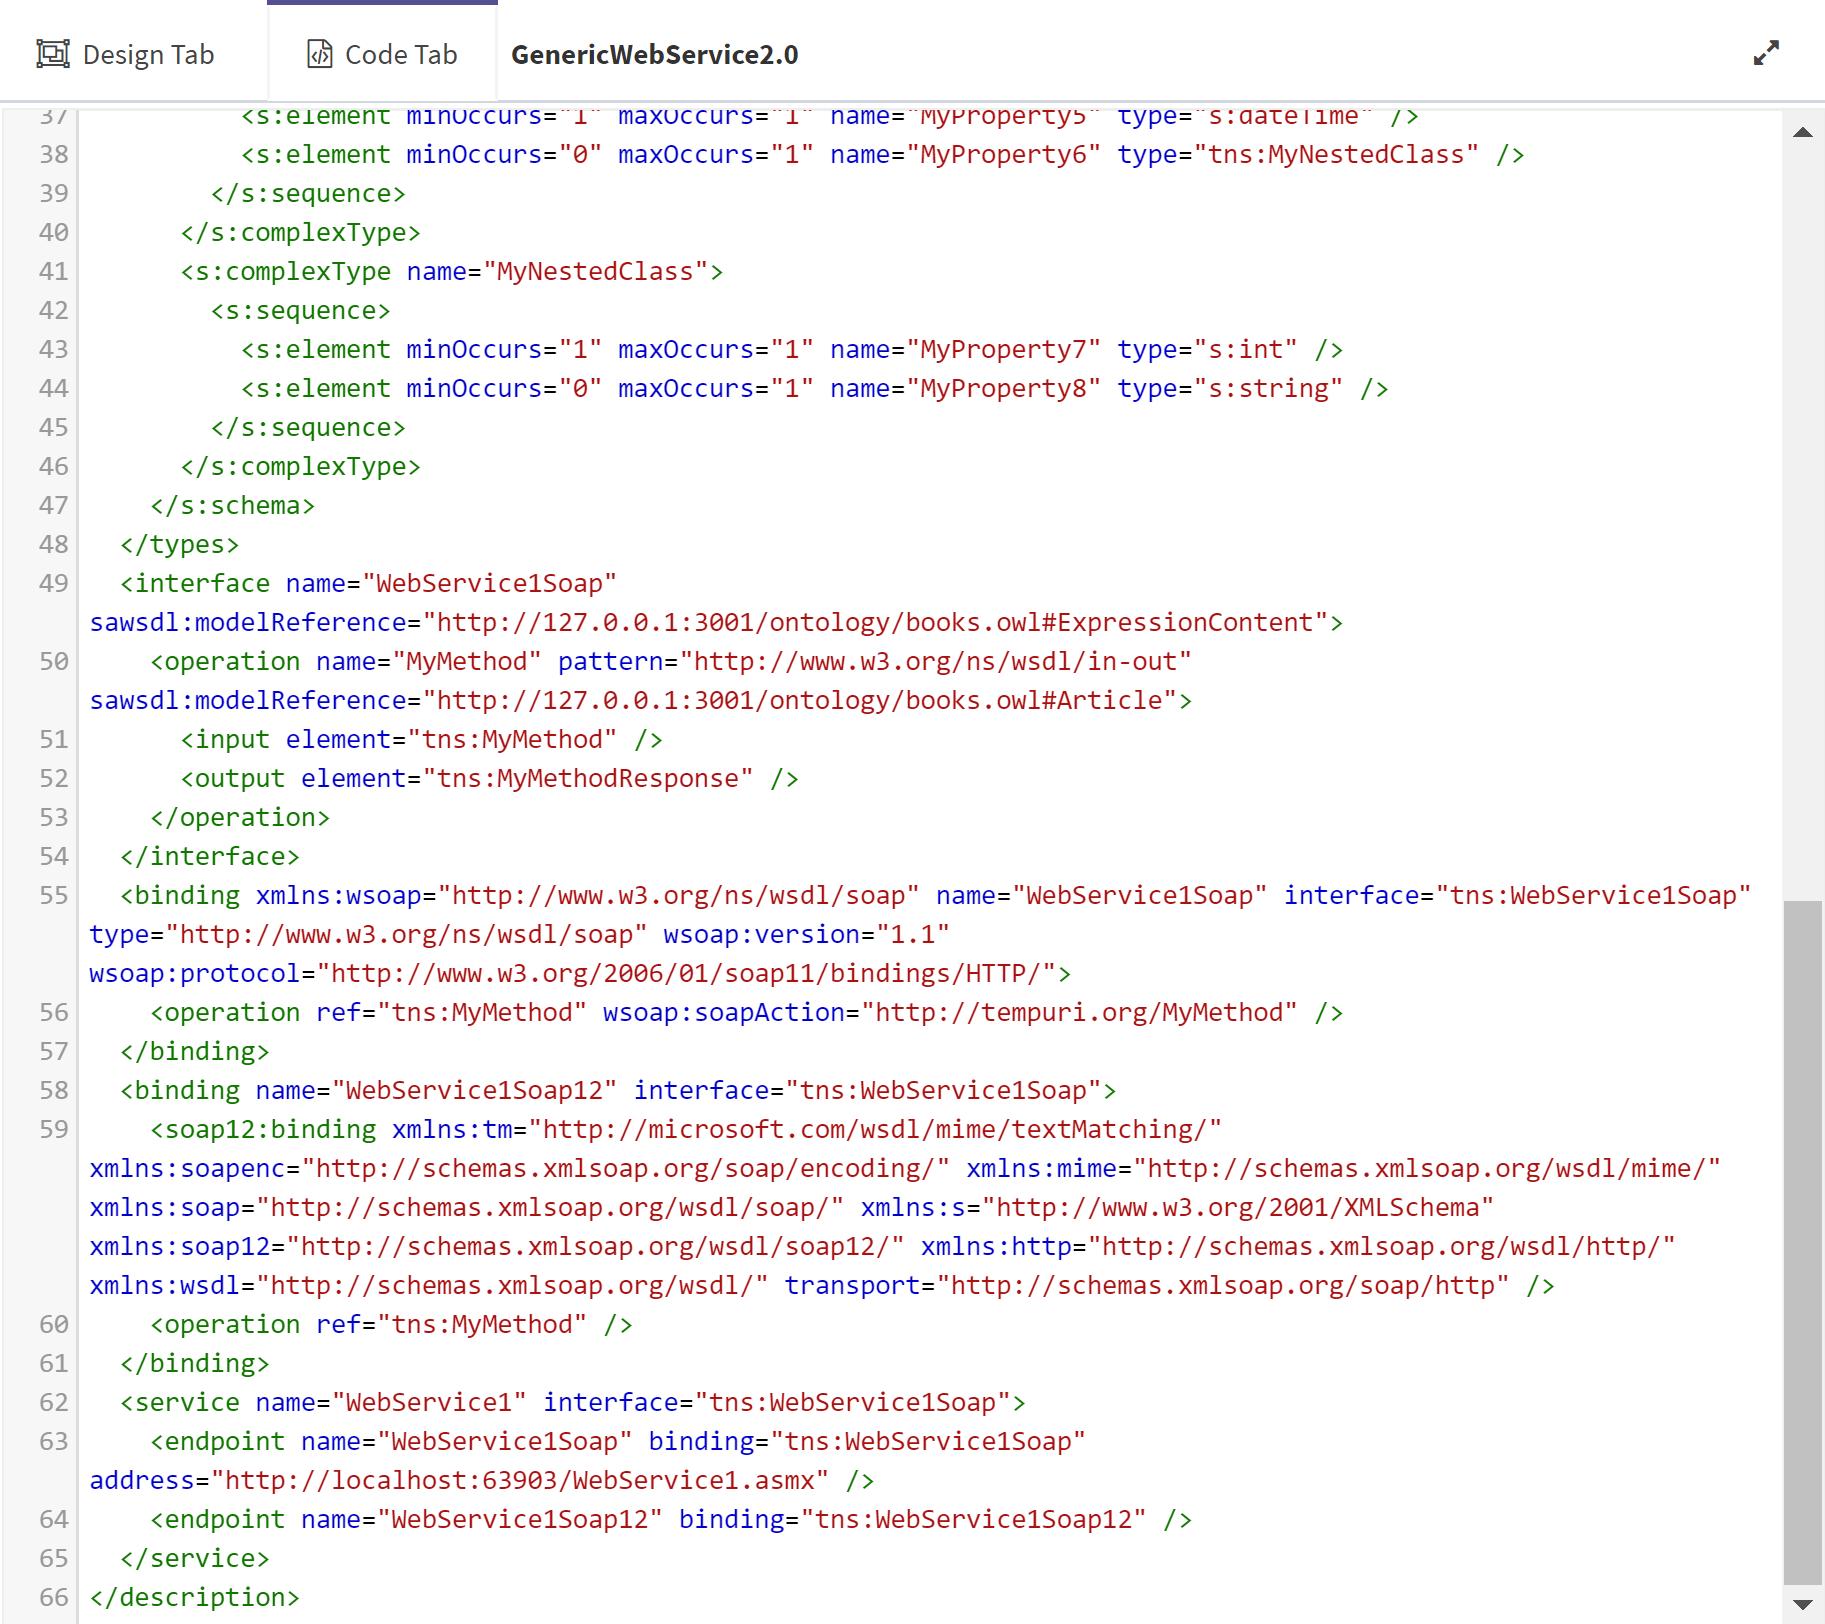
\includegraphics[scale=0.250]{4-grasews/imagens/grasews-painel-codigo.png}
    }
    \centering
    \caption[Painel de Grasews para visualização do código WSDL/XML]{\textbf{Painel de Grasews para visualização do código WSDL/XML.}}
    \label{fig:grasews-painel-codigo}
\end{figure}
\section{Menu \textit{tree-view}}\label{4-grasews-menu-tree-view}

Grasews utiliza um menu no formato de árvore (\textit{tree-view}) para auxiliar na compreensão tanto de uma especificação WSDL quanto de uma ontologia OWL, facilitando, consequentemente, o processo de anotação semântica.

\subsection{Menu \textit{tree-view} WSDL}\label{4-menu-wsdl}

De forma análoga ao grafo WSDL, o menu \textit{tree-view} de uma especificação WSDL também é composto por cinco níveis. Cada nível está diretamente associado ao nível correspondente do grafo WSDL. A \figurename~\ref{fig:menu-tree-view-wsdl} ilustra a estrutura hierárquica de elementos de uma especificação WSDL por meio do menu \textit{tree-view}. Esta estrutura permite identificar as relações de composição entre os diferentes tipos de elementos.

\begin{figure}[h]
    \resizebox{\textwidth}{!}{
        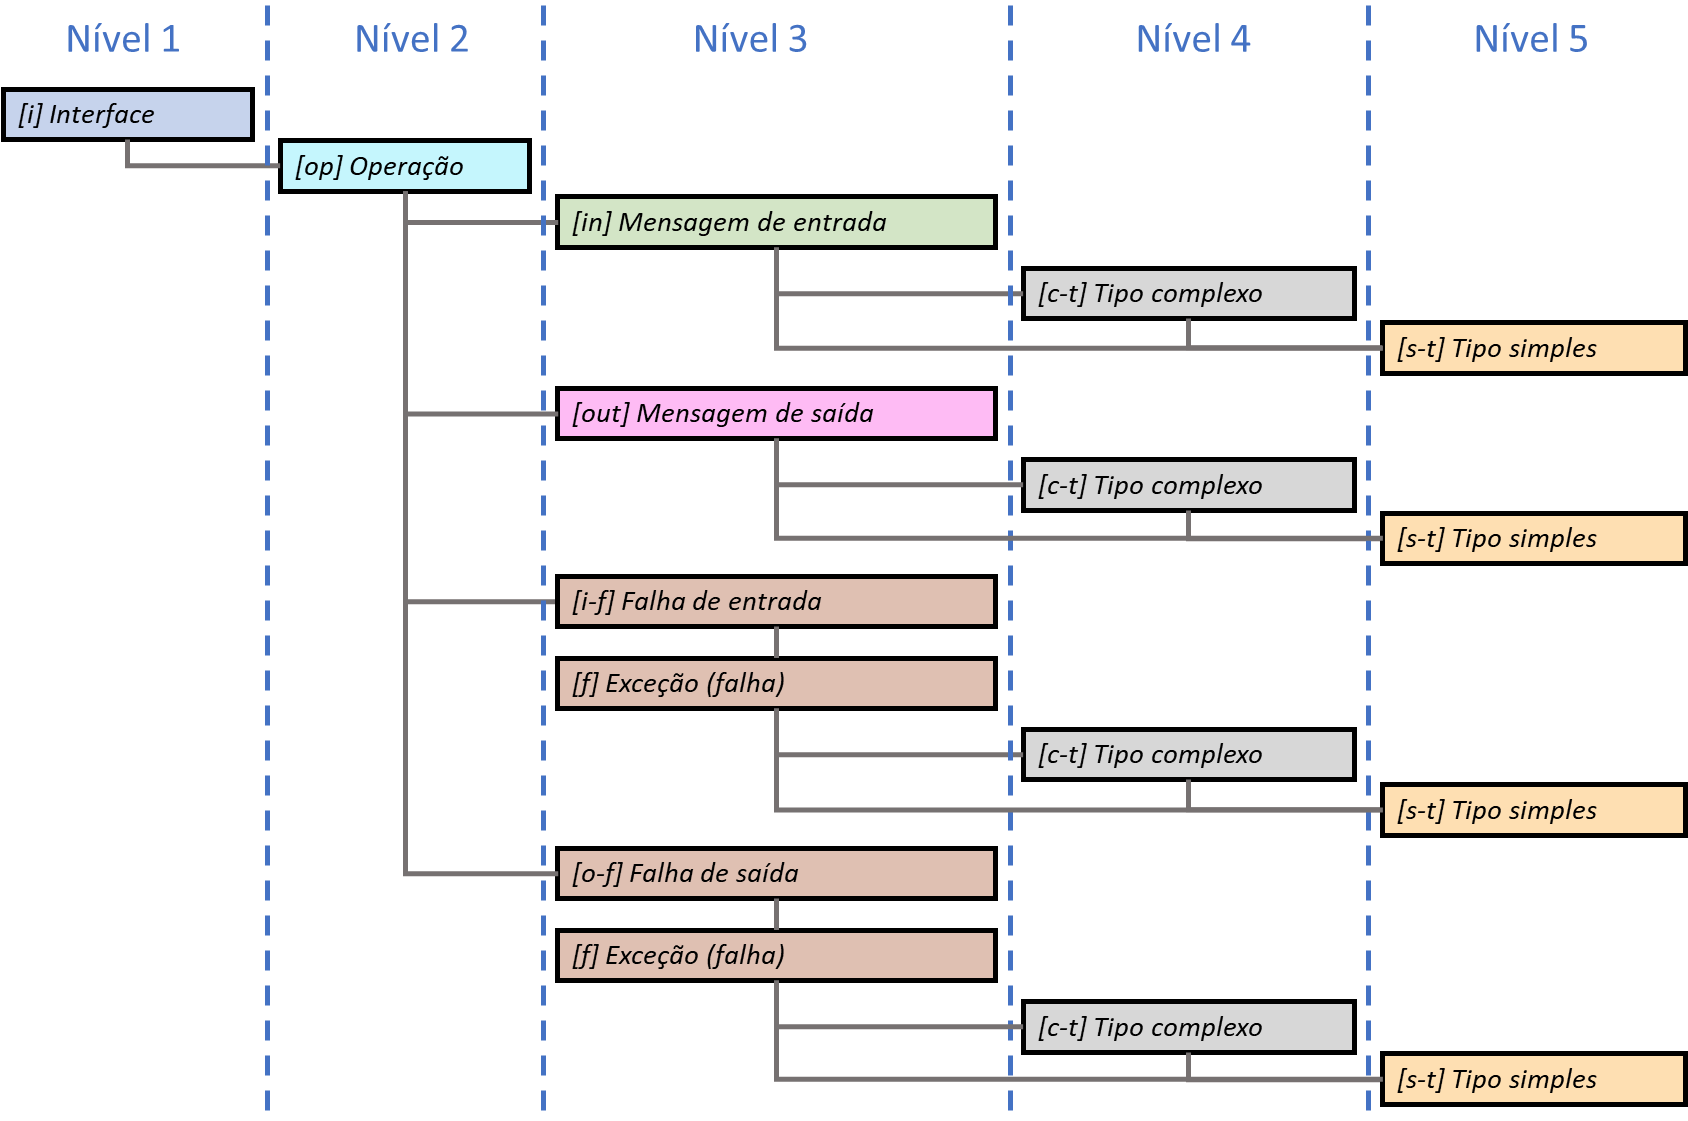
\includegraphics[scale=1]{4-grasews/imagens/menu-tree-view-wsdl.png}
    }
    \centering
    \caption[Estrutura da representação visual do menu \textit{tree-view} para uma especificação WSDL]{\textbf{Estrutura da representação visual do menu \textit{tree-view} para uma especificação WSDL.}}
    \label{fig:menu-tree-view-wsdl}
\end{figure}

No primeiro nível (nível 1), encontram-se os elementos do tipo \textit{wsdl:interface}. Estes elementos estão representados na cor azul para facilitar a associação com elementos do grafo que representam uma interface, também na cor azul. Adicionalmente, um elemento do tipo \textit{wsdl:interface} possui o prefixo \texttt{[i]} no menu \textit{tree-view}.

No segundo nível (nível 2), encontram-se os elementos do tipo \textit{wsdl:operation}. Estes elementos estão representados na cor ciano para facilitar a associação com elementos do grafo que representam uma operação, também na cor ciano. Adicionalmente, um elemento do tipo \textit{wsdl:operation} possui o prefixo \texttt{[op]} no menu \textit{tree-view}.

No terceiro nível (nível 3), encontram-se os elementos dos tipos \textit{wsdl:input}, \textit{wsdl:output}, \textit{wsdl:infault}, \textit{wsdl:outfault} e, finalmente, \textit{wsdl:fault}. Elementos \textit{wsdl:input} são representados na cor verde para facilitar a associação com elementos do grafo que representam uma mensagem de entrada, também na cor verde. Adicionalmente, um elemento \textit{wsdl:input} possui o prefixo \texttt{[in]} no menu. Elementos \textit{wsdl:output} são representados na cor rosa para facilitar a associação com elementos do grafo que representam uma mensagem de saída, também na cor rosa. Adicionalmente, um elemento \textit{wsdl:input} possui o prefixo \texttt{[out]} no menu. Por fim, elementos relacionados a falhas (exceções) são representados na cor marrom para facilitar a associação com elementos do grafo que representam uma mensagem de falha de entrada (\textit{wsdl:infault}), uma mensagem de falha de saída (\textit{wsdl:outfault}) ou, então, uma falha (\textit{wsdl:fault}), todos na cor marrom. Adicionalmente, um elemento \textit{wsdl:infault} possui o prefixo \texttt{[i-f]}, um elemento \textit{wsdl:outfault} possui o prefixo \texttt{[o-f]} e, finalmente, um elemento \textit{wsdl:fault} possui o prefixo \texttt{[f]}.

No quarto nível (nível 4), encontram-se os elementos do tipo \textit{xs:complexType}. Elementos \textit{xs:complexType} são representados na cor cinza para facilitar a associação com elementos do grafo que representam um tipo complexo, também na cor cinza. Adicionalmente, um elemento \textit{xs:complexType} possui o prefixo \texttt{[c-t]} no menu \textit{tree-view}.

Finalmente, no quinto nível (nível 5), encontram-se os elementos do tipo \textit{xs:simpleType}. Elementos \textit{xs:simpleType} são representados na cor laranja para facilitar a associação com elementos do grafo que representam um tipo simples, também na cor laranja. Adicionalmente, um elemento \textit{xs:simpleType} possui o prefixo \texttt{[s-t]} no menu \textit{tree-view}.

A \figurename~\ref{fig:grasews-menu-tree-view-wsdl} ilustra o menu \textit{tree-view} para uma especificação WSDL aberta na ferramenta Grasews. Inicialmente, ao abrir um documento WSDL na ferramenta, o menu \textit{tree-view} possui apenas o elemento \textit{wsdl:interface} visível. Conforme a navegação pelo menu \textit{tree-view}, o usuário pode descobrir elementos da especificação WSDL. Por meio das setas na lateral direita do menu, o usuário pode visualizar sub-elementos do menu, i.e., visualizar os elementos WSDL/XSD que compõem hierarquicamente uma especificação WSDL.  Uma seta orientada para a direita representa um item de menu que contém sub-itens, porém eles estão fechados, como, por exemplo, o item de menu \texttt{[in] MyMethod}. Uma seta orientada para baixo representa um item de menu que contém sub-itens e eles estão abertos, como, por exemplo os itens de menu \texttt{[i] WebService1Soap}, \texttt{[op] MyMethod}, \texttt{[out] MyMethodResponse}, \texttt{[c-t] MyMethodResponse}, \texttt{[c-t] MyClass} e \texttt{[c-t] MyNestedClass}. Por fim, quando um item de menu não possui sub-itens, não haverá seta para este item, como, por exemplo, todos os itens de menu que representam tipos simples XSD, i.e., todos os elementos com o prefixo \texttt{[s-t]}.

\begin{figure}[h]
    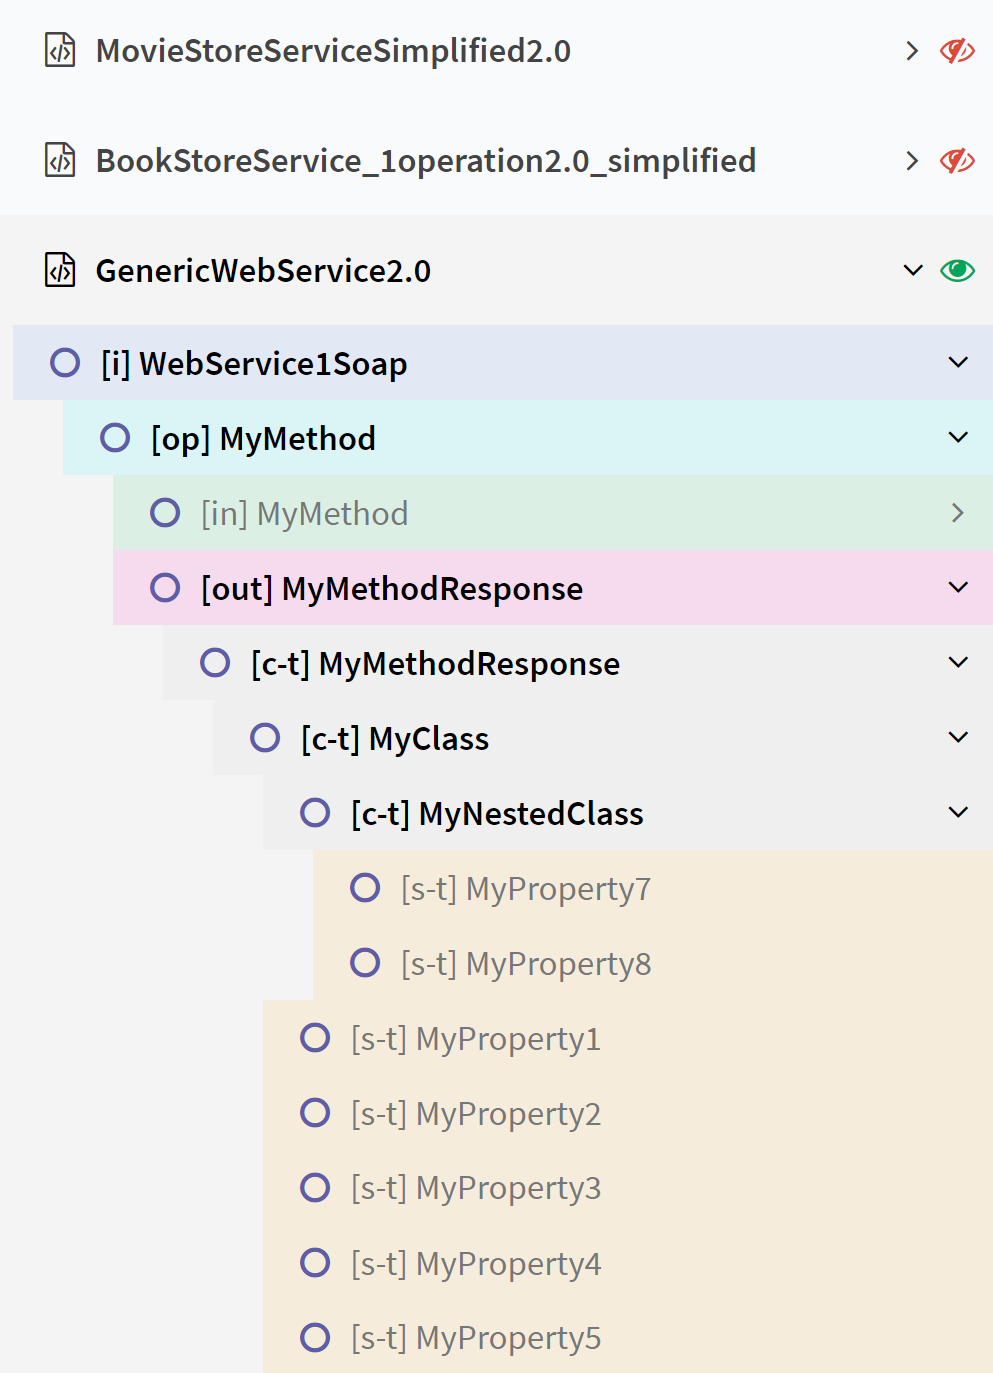
\includegraphics[scale=0.7]{4-grasews/imagens/grasews-menu-tree-view-wsdl.png}
    \centering
    \caption[Menu \textit{tree-view} de Grasews para uma especificação WSDL]{\textbf{Menu \textit{tree-view} de Grasews para uma especificação WSDL.}}
    \label{fig:grasews-menu-tree-view-wsdl}
\end{figure}

Grasews permite que múltiplos documentos WSDL sejam abertos simultaneamente, porém, apenas uma especificação WSDL pode ser visualizada no grafo por vez. A \figurename~\ref{fig:grasews-menu-tree-view-wsdl} ilustra os dois ícones utilizados pela ferramenta para indicar qual especificação WSDL está sendo vista ou não no grafo. O ícone com um olho verde indica que a especificação \texttt{GenericWebService2.0} encontra-se visível no grafo para o usuário, enquanto que o ícone com o olho vermelho cortado indica que as especificações \texttt{MovieStoreServiceSimplfied2.0} e \texttt{BookStoreService\_1operation2.0\_simplified} não estão visíveis no grafo para o usuário.

O menu \textit{tree-view} de uma especificação WSDL provê funcionalidades para o processo de anotação semântica. A \figurename~\ref{fig:grasews-menu-tree-view-icones-anotacao} ilustra o menu de contexto e as notações visuais (ícones) que auxiliam na anotação semântica de uma especificação WSDL.

\begin{figure}[h]
    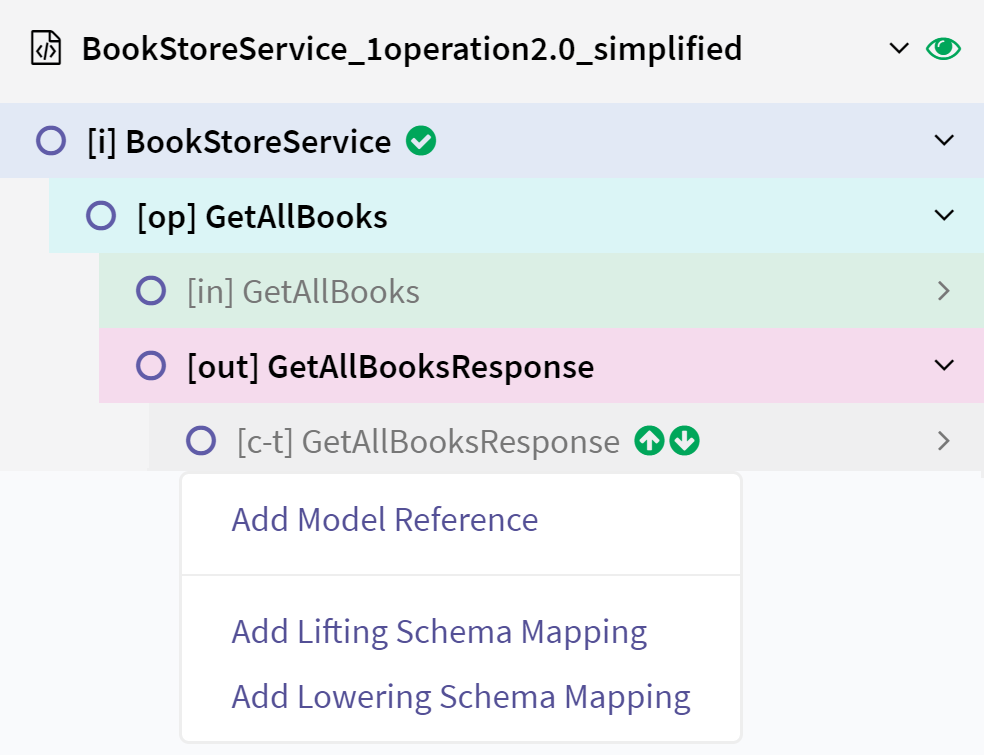
\includegraphics[scale=0.4]{4-grasews/imagens/grasews-menu-tree-view-icones-anotacao.png}
    \centering
    \caption[Menu \textit{tree-view} de Grasews para uma especificação WSDL]{\textbf{Menu \textit{tree-view} de Grasews para uma especificação WSDL.}}
    \label{fig:grasews-menu-tree-view-icones-anotacao}
\end{figure}

O menu \textit{tree-view} WSDL utiliza três ícones que indicam com qual atributo da anotação semântica um elemento WSDL/XSD está anotado. Na \figurename~\ref{fig:grasews-menu-tree-view-icones-anotacao}, o ícone com a marca de checagem, na lateral direita do elemento \texttt{[i] BookStoreService}, indica o uso do atributo \textit{Model Reference}. O ícone com a seta para cima, na lateral direita do elemento \texttt{[c-t] GetAllBooksResponse}, indica o uso do atributo \textit{Lifting Schema Mapping}. Finalmente, o ícone com a seta para baixo, também na lateral direita do elemento \texttt{[c-t] GetAllBooksResponse}, indica o uso do atributo \textit{Lowering Schema Mapping}.

Os elementos WSDL/XSD passíveis de anotação semântica segundo o padrão SAWSDL disponibilizam menus de contexto que podem ser acionados por meio do botão direito do \textit{mouse}. A \figurename~\ref{fig:grasews-menu-tree-view-icones-anotacao} ilustra um exemplo de menu de contexto para a anotação semântica. Quando o elemento WSDL/XSD é passível de ser anotado apenas com \textit{Model Reference}, o menu de contexto disponibiliza apenas a funcionalidade de adicionar \textit{Model Reference}. Quando o elemento WSDL/XSD já está anotado com \textit{Model Reference}, o menu de contexto de um elemento WSDL/XSD provê a funcionalidade de remoção da anotação semântica. Note que, como é possível ter múltiplos URIs para \textit{Model Reference}, a funcionalidade de adicionar \textit{Model Reference} continuará disponível para o usuário. Adicionalmente, a funcionalidade de remover \textit{Model Reference} também continuará disponível até que todos os URIs de \textit{Model Reference} sejam removidos do elemento.

Quando um elemento WSDL/XSD também é passível de ser anotado com \textit{Lifting Schema Mapping} e \textit{Lowering Schema Mapping}, o menu de contexto disponibiliza funcionalidades tanto para adicionar um URI para \textit{Lifting Schema Mapping} quanto para adicionar um URI para \textit{Lowering Schema Mapping}. Quando já anotado com \textit{Lifting Schema Mapping}, o menu de contexto de um elemento XSD provê a funcionalidade de remoção da anotação semântica. Note que, como é possível ter apenas um atributo \textit{Lifting Schema Mapping}, a funcionalidade de adicionar \textit{Lifting Schema Mapping} está indisponível para o usuário quando o elemento já está anotado com \textit{Lifting Schema Mapping}. O mesmo se aplica para \textit{Lowering Schema Mapping}.
\subsection{Menu \textit{tree-view} OWL}\label{4-menu-owl}

Adicionalmente, propusemos o uso de um menu \textit{tree-view} para auxiliar na compreensão das classes OWL passíveis de serem utilizadas na anotação semântica por meio do atributo \textit{Model Reference} de SAWSDL. A representação do menu \textit{tree-view} para classes de uma ontologia OWL facilita a identificação da hierarquia entre as classes OWL. Classes de conceitos mais genéricos encontram-se mais próximas à classe na raiz da árvore enquanto que classes de conceitos mais específicos encontram-se mais próximas das folhas da árvore. No menu \textit{tree-view} OWL, todas as classes OWL são representadas, independentemente se são utilizadas em uma anotação semântica ou não.

A \figurename~\ref{fig:menu-tree-view-owl} ilustra o uso de duas classes hierarquicamente dispostas no menu \textit{tree-view}. No primeiro nível (nível 1), encontramos a classe base com um conceito mais genérico, enquanto que nos níveis inferiores (de nível 2 a nível N), encontramos as classes de conceitos mais específicos. Esta estrutura pode conter N níveis, dependendo da ontologia e a quantidade de especializações que pode existir entre suas classes.

\begin{figure}[h]
    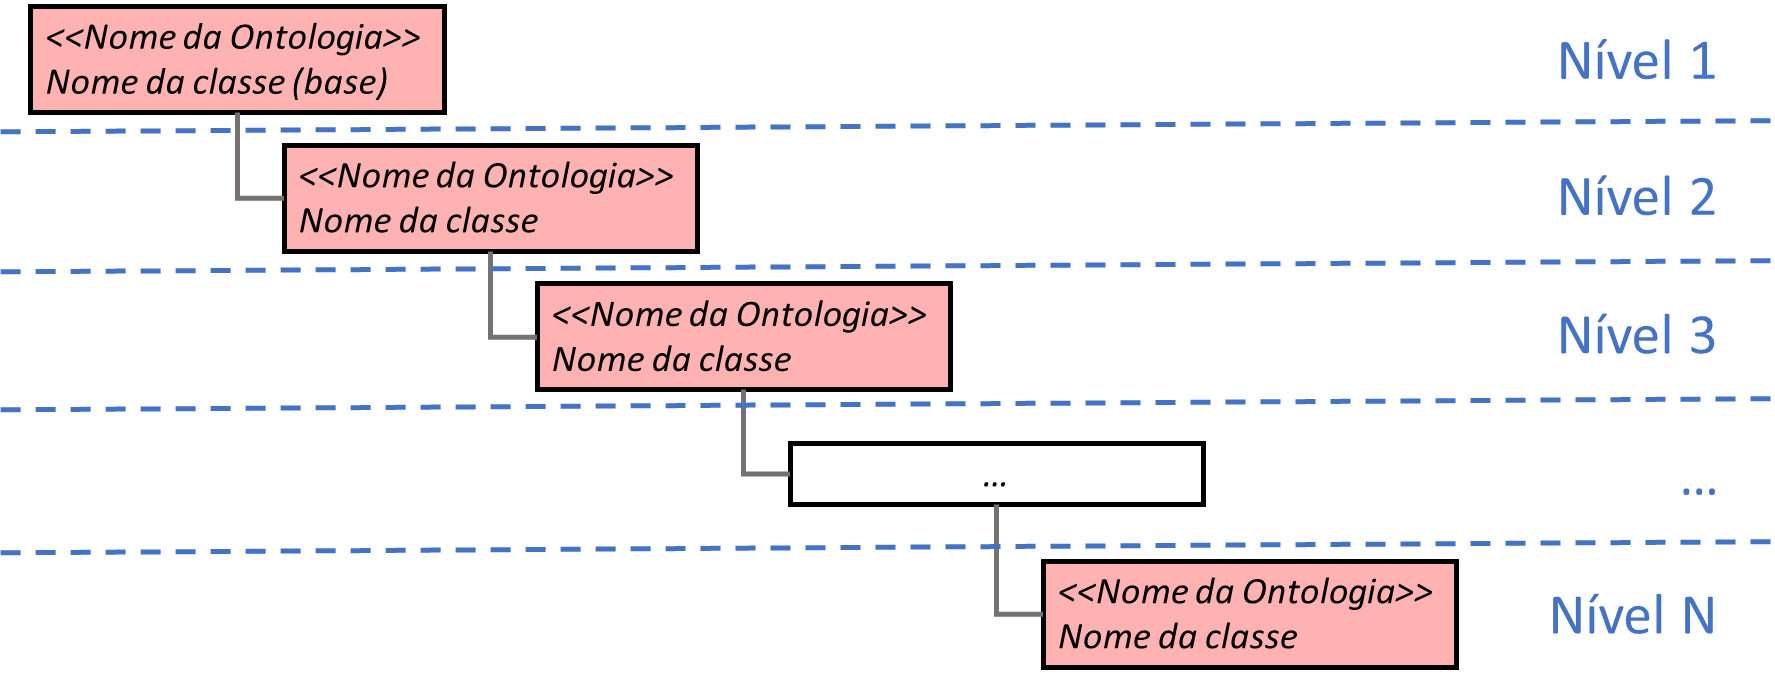
\includegraphics[scale=0.3]{4-grasews/imagens/menu-tree-view-owl.png}
    \centering
    \caption[Estrutura da representação visual do menu \textit{tree-view} para uma ontologia OWL]{\textbf{Estrutura da representação visual do menu \textit{tree-view} para uma ontologia OWL.}}
    \label{fig:menu-tree-view-owl}
\end{figure}

O menu \textit{tree-view} OWL é localizado no painel direito de Grasews. O menu \textit{tree-view} de uma ontologia OWL também provê recursos para o processo de anotação semântica por meio de um menu de contexto. Assim como no menu \textit{tree-view} WSDL, o menu de contexto do menu \textit{tree-view} OWL pode ser acessado por meio do botão direito do \textit{mouse} em uma classe OWL do menu. A \figurename~\ref{fig:grasews-menu-owl-contexto} ilustra o menu de contexto associado à classe OWL \texttt{ExpressionContext} para a anotação com o atributo \textit{Model Reference}. Neste exemplo, Grasews possibilita que um usuário adicione um URI de \texttt{ExpressionContext} como atributo \textit{Model Reference} a um elemento de uma especificação WSDL que esteja visível no grafo da ferramenta. Para adicionar uma anotação semântica \textit{Model Reference} a partir de uma classe OWL do menu \textit{tree-view}, o usuário deve selecionar o elemento WSDL/XSD no qual a anotação semântica será adicionada.

\begin{figure}[h]
    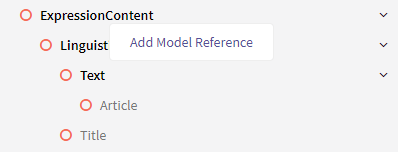
\includegraphics[scale=0.7]{4-grasews/imagens/grasews-menu-owl-contexto.png}
    \centering
    \caption[Menu de contexto para uma classe OWL no menu \textit{tree-view}]{\textbf{Menu de contexto para uma classe OWL no menu \textit{tree-view}.}}
    \label{fig:grasews-menu-owl-contexto}
\end{figure}